\documentclass[10pt,a4paper]{article}
\usepackage[utf8]{inputenc}
\usepackage{amsmath}
\usepackage{amsfonts}
\usepackage{amssymb}
\usepackage{graphicx}
\usepackage{usecases}
\usepackage{listings}
\usepackage{color}

\definecolor{mygreen}{rgb}{0,0.6,0}
\definecolor{mygray}{rgb}{0.5,0.5,0.5}
\definecolor{mymauve}{rgb}{0.58,0,0.82}

% Define colors used for listings
\definecolor{dkgreen}{rgb}{0,0.6,0}
\definecolor{gray}{rgb}{0.5,0.5,0.5}
\definecolor{mauve}{rgb}{0.58,0,0.82}
% Configuration for listings
\lstset{%
numbers=left,
frame=single,
basicstyle=\small,
numbers=left,
numberstyle=\tiny,
numbersep=15pt,tabsize=4,
flexiblecolumns=true,
keywordstyle=\color{blue},
commentstyle=\color{dkgreen},
stringstyle=\color{mauve},
numberstyle=\tiny\color{gray},
language=Java,
breaklines=true,
breakatwhitespace=true,
morekeywords={*,num,String,var,library,get,set} ,
}

\author{Kim Rostgaard Christensen}
\begin{document}

%Note: Domain concepts are usually also present in the mapping, and are usually mapped directly to a class.
\title{Use case translation concepts}
\maketitle
This section takes offset in an use case description, and tries to go through the steps needed to convert it into an acceptance tests. The use case used in this text is outlined below in verbatim text.
\begin{verbatim}
Scenario:
  Receptionist types in message
  Receptionist sends message
  Receptionist returns to ready state
Postconditions:
  The message is stored
  The receptionist is ready to handle the next call
\end{verbatim} 
The first thing that needs to be done is to identify the domain concept of the statements in the text. We observe that it includes the concept ``message'' a ``receptionist'' actor. There is also some interaction between the message and the actor, which we define as actions.\\
Highlighting the basics of the use case, using square brackets for domain concepts curly brackets for actions and regular parentheses for attributes, it looks like this:
\begin{verbatim}
Scenario:
  [receptionist] {types in} [message]
  [receptionist] {sends} [message]
  [receptionist] {returns to} [ready state]
Postconditions:
  The [message] (is stored)
  The [receptionist] (is ready) to handle the next call
\end{verbatim} 
Each of the concepts in this example is mapped to a class, that could likely be stubbed out automatically by the test tool.\\\\
Given the amount of information in (and markup of) the use cases, we can easily generate code such as the one shown in listing \ref{lst:uc2_example_test_code}. But these functions are still very high-level, and doesn't assert anything about the system being tested. To do this, we need to fill in the methods used on our receptionist and message object.
\begin{lstlisting}[caption=Generated test case,label={lst:uc2_example_test_code}]
boolean test (receptionist, message) {
  // Scenario
  receptionist.types_in (message);
  receptionist.sends (message);
  receptionist.returns_to (ready_state);
  
  // Postcondition
  return
    message.is_stored() AND
    receptionist.is_ready();
}
\end{lstlisting}
Going through the test case, from the top, we can see that the \texttt{receptionist.types\_in~(message)} method operates on the receptionist actor call, and requires knowledge of the ``message'' domain concept. Furthermore, we known from the domain analysis that \emph{is not part} of the use case, that the action of typing in a message is actually a creation of message. So, before being able to test it, we need some way of simulating the message creation and -- more concretely -- fill in the actual message content. Conceptually, this is some sort of content generator. A concrete implementation could be a simply ``dummy object'' or an object that is initialized with random content. Once the message object is mapped to a content generation function, we will be able to fully generate the test. The content generation function would probably still need to be hand coded, as this is example data.\\\\
The next statement; \texttt{receptionist.sends (message)} can be classified as a store function. It takes the argument ``message'' and makes it available for other actors to access later on, by storing it persistently. This is typically done using a database or file store. By mapping a message to a message store, we can remap an ``enqueue'' method of the message object, which needs to have a notion of where it is, or should be stored. This is realized by having a ``messageStore'' interface which is a service interface object that, can actually be originating directly from the code base of the system under test.\\\\
The final statement in the scenario is \texttt{receptionist.returns\_to (ready\_state)}. This is actually a mutation function that alters the state of the receptionist actor. This state change could be global and should then  be updated multiple places, which then leads to additional ``state-store'' dependencies. Here, we also note that there is a concept of a ready\_state this is an explicit state change that could, possibly be linked to a state machine contained within the receptionist actor object.\\\\
The final thing done in the tests, is the postconditions. In this case, we treat the postcondition as a boolean attribute of the concept which it refers to. The general assumption is that pre- and postconditions are expressions that must always be true, and must refer to a concept previously referred to in the scenario. So for the \texttt{receptionist.is\_ready()} predicate we can map it to the internal state of the receptionist being equal to the ``ready'' state.\\\\
The mapping can be described in a textual language such as shown in listing \ref{lst:mapping_language_concept} where we initially state the domain concept name -- which is in this case Receptionist -- and the requirements, properties and mappings it has, plus which functionality it provides. The requirements are which other domain concepts are needed by this one. The properties are the boolean properties that are used in predicates and the ``provides'' section are functions that are either used as internal auxiliary functions, or exported functions that other concepts may use.
%Prior to running the tests, the two objects ``message'' and ``receptionist'' needs to be initialized.
%The question is then how much more needs to be added. Can we use some stereotyping to increase the semantics of the annotated use cases? Such as 'storage' for message, and 'actor' for receptionist.
%So last question; who does what, and how much can be automated?
%The first part of the job; typing in the use cases is a manual process that should be done in close cooperation with -- and preferably by -- the stakeholder involved in the use case. So a use case involving an accountant actor should be typed by a accountant representative expected to be using the system, once finished.

\begin{lstlisting}[caption=example language for mapping concepts,label={lst:mapping_language_concept}]:
Receptionist:
  requires:
    MessageContentGenerator messageContentGenerator
    ReceptionistState currentState = ReceptionistState.Unknown
  
  provides:
    changeState (ReceptionistState rs) -> currentState = rs
  
  maps:
    sends_message (Message msg) -> msg.enqueue()
    types_in (Message msg) -> msg.content = messageContentGenerator.next().content
    returns_to (ReceptionistState newState) -> this.changeState (newState)

  properties:
    is_ready -> receptionistState == ready
\end{lstlisting}
The mappings are, in this conceptual model, alias functions to ``real methods'' already provided in the code base of the software under tests, or to functions of other domain concepts. This is probably not feasible in praxis, and will probably be a programing code template instead.

\begin{lstlisting}[caption=Pseudo code representing Receptionist domain actor,label={lst:code_for_receptionist_domain_actor}]
class Receptionist {
   MessageContentGenerator messageContentGenerator= ...;
   ReceptionistState receptionistState = ...;
  
  void types_in (message) {
  	message.updateContent(messageContentGenerator.content);
  }
  
  void sends (Message message) {
    message.enqueue();
  }
  
  // Alias function.
  void returns_to (State newState) {
  	changeState (newState);
  }
  
  void changeState (State newState){
  	receptionistState = newState;
  }
  
  boolean is_ready() {
    return receptionistState == ready;
  }
}
\end{lstlisting}

\begin{lstlisting}[caption=Pseudo code representing Message domain concept,label={lst:code_for_domain_concept}]
class Message {
  MessageStore messageStore = ...;
  
  void enqueue() {
    messageStore.enqueue(message);
  }

  boolean message.is_stored() {
    messageStore.contains(this);
  }
}
\end{lstlisting}

\begin{figure}
 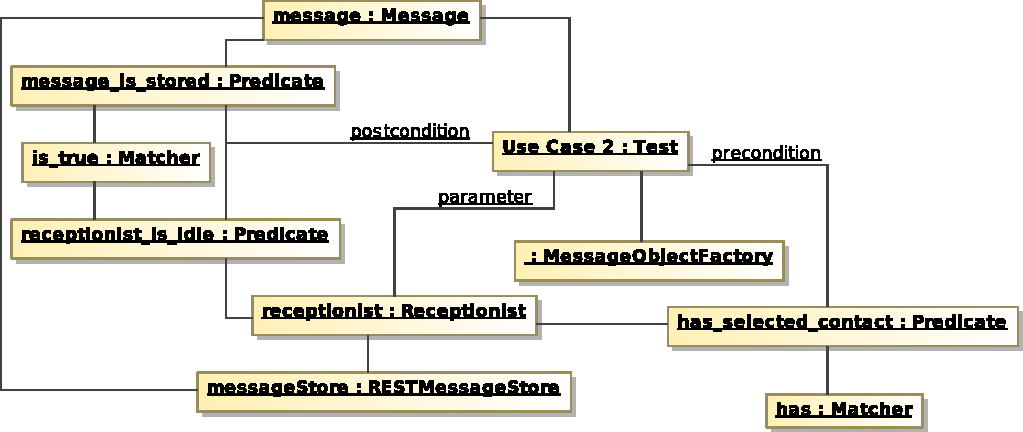
\includegraphics[scale=0.45]{img/uc2_test_config}
 \caption{Object diagram showing the use case as mapped test}
\end{figure}
\end{document}